\documentclass[12pt,a4paper,twoside]{article}
\usepackage[a4paper,left=25mm,right=25mm,bottom=25mm,top=25mm]{geometry}
\usepackage[T1]{fontenc}
\usepackage{lmodern}
\usepackage[british]{babel}
\usepackage{amsmath,amssymb,graphicx,booktabs,array,tabularx,fancyhdr}
\usepackage[square,comma,numbers,sort&compress]{natbib}
\usepackage[hidelinks]{hyperref}
\usepackage{caption}
\usepackage{microtype}
\graphicspath{{figures/}{./}}
\captionsetup{font=small,labelfont=bf,justification=raggedright,singlelinecheck=false}
\setlength{\parindent}{0em}
\setlength{\parskip}{0.3em}
\setlength{\headheight}{15pt}
\setlength{\emergencystretch}{1em}
\renewcommand{\topfraction}{0.92}
\renewcommand{\bottomfraction}{0.85}
\renewcommand{\textfraction}{0.05}
\renewcommand{\floatpagefraction}{0.85}
\setcounter{topnumber}{3}
\setcounter{bottomnumber}{2}
\setcounter{totalnumber}{4}
\setlength{\textfloatsep}{12pt plus 2pt minus 2pt}
\setlength{\floatsep}{10pt plus 2pt minus 2pt}
\setlength{\intextsep}{10pt plus 2pt minus 2pt}
\makeatletter
\setlength{\@fptop}{0pt}
\setlength{\@fpsep}{16pt}
\makeatother
\pagestyle{fancy}
\fancyhead{}
\fancyhead[C]{\small Lab 4: Trajectory optimisation and drone racing}
\fancyfoot{}
\fancyfoot[C]{\thepage}
\renewcommand{\headrulewidth}{0pt}
\renewcommand{\footrulewidth}{0pt}
\renewcommand{\abstractname}{Summary}
% Author, student number, lab group, experiment date and contributions are deferred.
\newcommand{\studentname}{Author details to be completed}
\title{Lab 4 Report\\[0.3em]\large Trajectory optimisation and drone racing}
\author{\studentname}
\date{Report date: 10 October 2026}
\hypersetup{pdftitle={Lab 4 Report: Trajectory optimisation and drone racing},pdfauthor={}}

\begin{document}
\raggedbottom
\renewcommand{\abstractname}{Summary}
\maketitle
\begin{abstract}
Polynomial trajectory optimisation connects waypoint geometry to the continuous
state references required for quadrotor flight. This laboratory derives the
single-segment minimum-velocity solutions, counts the conditions for multi-segment
minimum-snap trajectories, and implements a ROS trajectory follower for the official
Unity racing course. With endpoint positions alone, the optimum is $P(t)=t$ and its
cost is 1 for all three polynomial degrees considered. A prescribed terminal velocity
changes the solution: the cubic reduces the quadratic cost from 4 to $17/8$.
In the recorded Unity run, the quadrotor approached all 12 gate centres in order
while tracking a 91.08\,s reference trajectory. The active-flight position error
had a root-mean-square (RMS) value of 0.319\,m, and the final position was 0.169\,m from the last gate centre.
\end{abstract}

\section{Lab introduction and team information}
The task is to convert a sequence of gate poses into a smooth flight reference and
track it through the official simulated course. The exercises combine two analytical
deliverables with a drone-racing implementation\cite{lab4}. This report follows that
sequence: quadratic programming explains how endpoint constraints shape a polynomial;
multi-segment analysis explains how adjacent pieces join; the flight experiment
shows how the resulting reference interacts with a feedback controller.

The implemented system is shown in Figure~\ref{fig:system}. Gate positions and orientations
are supplied by the course map. The trajectory generator produces desired states,
and the controller from Lab 3 closes the loop through the TESSE bridge. Team names,
student numbers, group information and individual contributions will be added after
the author details are confirmed.

\begin{figure}[!htbp]
\centering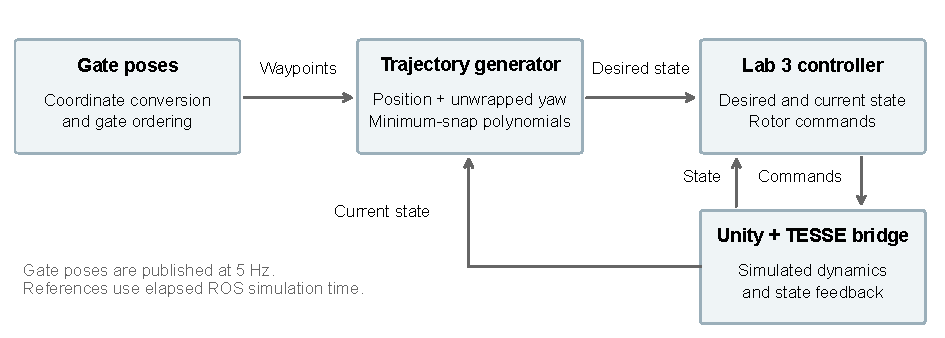
\includegraphics[width=\linewidth]{system_overview.pdf}
\caption{Implemented ROS control loop. Gate poses enter the generator on
\texttt{/desired\_traj\_vertices}; the generator publishes
\texttt{/desired\_state}, and feedback arrives on \texttt{/current\_state}.
Arrows show command and feedback interfaces.}
\label{fig:system}
\end{figure}

\section{Individual work}
\subsection{Deliverable 1: single-segment trajectory optimisation}
The objective is to minimise squared velocity on the normalised interval $[0,1]$:
\begin{equation}
\min_P J(P)=\int_0^1[P'(t)]^2\,dt,
\qquad P(0)=0,\quad P(1)=1.
\label{eq:single}
\end{equation}
Write $P(t)=\sum_{i=1}^N p_i t^i$. The constant coefficient is zero because
$P(0)=0$. With $\boldsymbol p=[p_1,\ldots,p_N]^T$, direct integration gives
\begin{equation}
J=\boldsymbol p^TQ\boldsymbol p,\qquad Q_{ij}=\frac{ij}{i+j-1},\qquad
A\boldsymbol p=b,\quad A=[1,\ldots,1],\quad b=1.
\label{eq:qp}
\end{equation}
$Q$ is positive definite: a nonzero coefficient vector gives a nonzero derivative
polynomial and hence a strictly positive integral of its square. Thus each feasible
equality-constrained problem has a unique minimum. A solver that defines the objective
as $\tfrac12\boldsymbol p^TH\boldsymbol p$ must use $H=2Q$.

\subsubsection{Question 1: degree one}
For $P(t)=p_1t$, the endpoint equation fixes $p_1=1$. Therefore
\begin{equation}
\boxed{P^*(t)=t,\qquad J^*=1.}
\end{equation}

\subsubsection{Question 2: degree two}
For $P(t)=p_2t^2+p_1t$, the requested matrices and objective are
\begin{equation}
Q=\begin{bmatrix}1&1\\1&4/3\end{bmatrix},\quad
A=\begin{bmatrix}1&1\end{bmatrix},\quad b=1,
\qquad J=p_1^2+2p_1p_2+\frac43p_2^2.
\end{equation}
Substituting $p_1=1-p_2$ gives $J=1+\tfrac13p_2^2$. The optimum is
$\boldsymbol p^*=(1,0)^T$, so $P^*(t)=t$ and $J^*=1$. The quadratic term
provides no cost reduction for these boundary conditions.

\subsubsection{Question 3: degree three and the Euler--Lagrange equation}
For $P(t)=p_3t^3+p_2t^2+p_1t$,
\begin{equation}
Q=\begin{bmatrix}1&1&1\\1&4/3&3/2\\1&3/2&9/5\end{bmatrix},\quad
A=\begin{bmatrix}1&1&1\end{bmatrix},\quad b=1.
\end{equation}
The Karush--Kuhn--Tucker (KKT) equations,
\begin{equation}
2Q\boldsymbol p+A^T\lambda=0,\qquad A\boldsymbol p=b,
\end{equation}
give $\boldsymbol p^*=(1,0,0)^T$ and $\lambda=-2$. Again $J^*=1$.
For the integrand $(P')^2$, the Euler--Lagrange equation is $P''=0$,
which yields the same linear trajectory. Cauchy--Schwarz also gives the global bound
\begin{equation}
J\geq\left(\int_0^1P'(t)\,dt\right)^2=[P(1)-P(0)]^2=1.
\end{equation}
Equality requires constant velocity, so increasing the degree cannot improve this result.

\subsubsection{Question 4: prescribed terminal velocity}
Adding $P'(1)=-2$ supplies a second constraint row, $[1,2,\ldots,N]$,
with $b=(1,-2)^T$. The equality-constrained minimum can be written as
\begin{equation}
\boldsymbol p^*=Q^{-1}A^T(AQ^{-1}A^T)^{-1}b.
\end{equation}

For degree two,
\begin{equation}
A=\begin{bmatrix}1&1\\1&2\end{bmatrix},\quad
b=\begin{bmatrix}1\\-2\end{bmatrix},\quad
\boldsymbol p^*=\begin{bmatrix}4\\-3\end{bmatrix}.
\end{equation}
Both coefficients are fixed by the constraints, giving
\begin{equation}
\boxed{P^*(t)=4t-3t^2,\qquad J^*=\int_0^1(4-6t)^2\,dt=4.}
\end{equation}

For degree three,
\begin{equation}
A=\begin{bmatrix}1&1&1\\1&2&3\end{bmatrix},\qquad
b=\begin{bmatrix}1\\-2\end{bmatrix}.
\end{equation}
Set $p_3=z$. The constraints give $p_1=4+z$ and $p_2=-3-2z$, so
\begin{equation}
J(z)=4+z+\frac{2}{15}z^2,\qquad J'(z)=1+\frac{4}{15}z.
\end{equation}
Its minimum occurs at $z=-15/4$, with
\begin{equation}
\boxed{P^*(t)=\frac14t+\frac92t^2-\frac{15}{4}t^3,\qquad J^*=\frac{17}{8}.}
\end{equation}
The cubic satisfies both $P(1)=1$ and $P'(1)=-2$. Its additional freedom reduces
the integrated squared velocity by $46.875\%$ relative to the quadratic. Both
trajectories overshoot the final position before returning with negative velocity
(Figure~\ref{fig:single}). These solutions minimise the cost within their specified
polynomial spaces; the linear Euler--Lagrange solution cannot satisfy the added
terminal-velocity condition.

\begin{figure}[!htbp]
\centering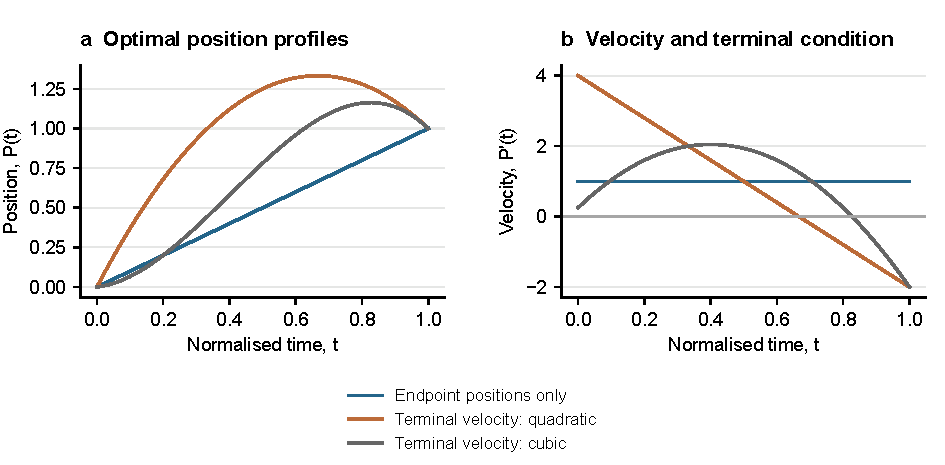
\includegraphics[width=\linewidth]{single_segment.pdf}
\caption{Exact solutions of the single-segment exercises. (a) Position profiles.
(b) Their analytic derivatives. The blue line solves the position-only problem
for degrees one, two and three. The other curves include $P'(1)=-2$; their
costs are 4 (quadratic) and $17/8$ (cubic). These are analytical curves,
not flight measurements.}
\label{fig:single}
\end{figure}

Figure~\ref{fig:objectives} shows the reduced objectives after the endpoint
equations have been eliminated. The stationary points of these one-dimensional
quadratics give the same coefficients as the matrix solution. In the terminal-velocity
problem, setting the cubic coefficient to zero recovers the degree-two solution.
\begin{figure}[!htbp]
\centering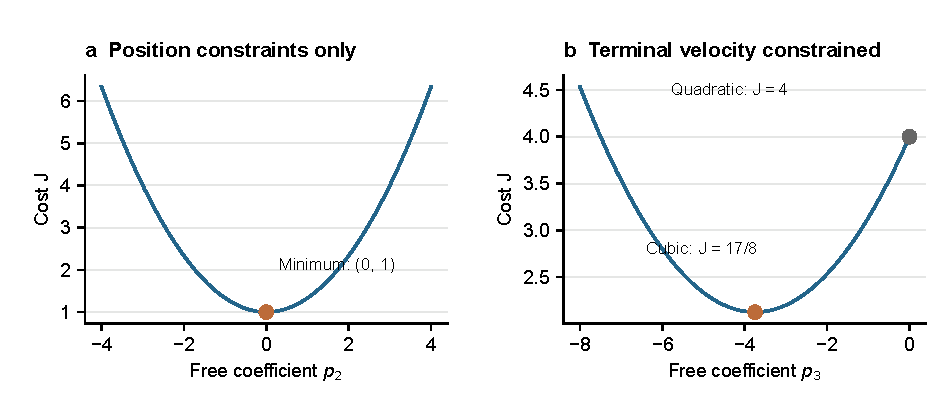
\includegraphics[width=\linewidth]{reduced_objectives.pdf}
\caption{The analytical cost landscapes. (a) For the position-only quadratic,
$J=1+p_2^2/3$ is minimised at $p_2=0$. (b) With terminal velocity $-2$,
the cubic's reduced objective is $J=4+p_3+2p_3^2/15$. Its minimum at
$p_3=-15/4$ has cost $17/8$; the point $p_3=0$ has the quadratic cost 4.}
\label{fig:objectives}
\end{figure}

\subsection{Deliverable 2: multi-segment trajectory optimisation}
All counts below refer to one scalar coordinate, prescribed waypoint positions and
fixed, strictly increasing knot times $t_0<\cdots<t_k$. Coordinates can be treated
independently when the cost is their summed squared derivative norm.

\subsubsection{Question 1: minimum snap}
For $k$ segments, the snap objective is
\begin{equation}
J=\sum_{i=1}^{k}\int_{t_{i-1}}^{t_i}[P_i^{(4)}(t)]^2\,dt.
\end{equation}
Euler--Lagrange gives $P_i^{(8)}=0$ on every open segment. Each piece therefore
has degree at most seven and eight coefficients, giving $8k$ unknowns.
Assume that position, velocity, acceleration and jerk are fixed at the overall
start and end. The conditions determining the stationary optimum are listed in
Table~\ref{tab:counts}.

\begin{table}[htbp]
\centering\small
\caption{Scalar condition count for $k$ minimum-snap segments. The free-derivative
row combines continuity constraints with natural optimality conditions.}
\label{tab:counts}
\begin{tabularx}{\linewidth}{@{}lXr@{}}
\toprule
Type & Conditions & Count\\\midrule
Waypoint & Fix both ends of each piece to the appropriate waypoint. & $2k$\\
Free derivative & Match derivatives of orders 1 to 6 across each interior knot. & $6(k-1)$\\
Fixed derivative & Specify orders 1 to 3 at the overall start and end. & $6$\\\midrule
Total & Eight conditions per polynomial piece. & $8k$\\\bottomrule
\end{tabularx}
\end{table}

There are $k+1$ physical waypoints. Each interior waypoint supplies two position
equations, one for each adjacent piece, while each overall endpoint supplies one.
For $k=3$, the counts are 6 waypoint, 12 free-derivative
and 6 fixed-derivative equations, totalling 24.

The derivative map in Figure~\ref{fig:continuity} shows where these conditions
act. Each interior position is imposed on both adjacent pieces, whereas the
free derivatives share a common value across the knot.
\begin{figure}[!htbp]
\centering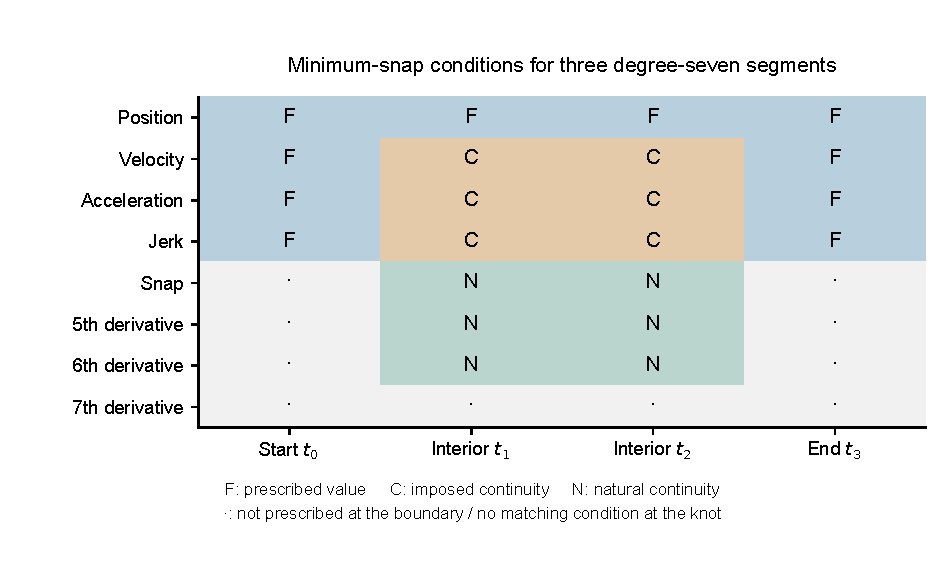
\includegraphics[width=\linewidth]{continuity_map.pdf}
\caption{Condition map for the theoretical three-segment minimum-snap problem.
F denotes a prescribed value, C an explicit continuity constraint and N a natural
continuity condition supplied by stationarity. Each interior F in the position row
represents two scalar equations. Dots identify derivative values that are not
prescribed at an endpoint, or derivatives with no knot-matching condition.}
\label{fig:continuity}
\end{figure}

Velocity, acceleration and jerk continuity define admissible trajectories. Their
common values at interior knots remain free. Minimising snap then supplies continuity
of derivatives four, five and six as natural optimality conditions. The seventh
derivative may jump because the interior positions are prescribed. Thus a QP
needs $2k+3(k-1)+6=5k+3$ explicit equality constraints; optimisation supplies the
remaining $3(k-1)$ conditions. Treating all $8k$ equations as prescribed derivative
values would remove the distinction between feasibility and optimality.

\subsubsection{Question 2: a general derivative order}
For an objective involving the squared $r$th derivative,
\begin{equation}
J=\sum_{i=1}^{k}\int_{t_{i-1}}^{t_i}[P_i^{(r)}(t)]^2\,dt,
\end{equation}
Euler--Lagrange gives $P_i^{(2r)}=0$. The degree is at most $2r-1$, with $2rk$
coefficients in total. Prescribe endpoint derivatives of orders $1,\ldots,r-1$.
The counts become
\begin{equation}
\boxed{\underbrace{2k}_{\text{waypoint}}
+\underbrace{(2r-2)(k-1)}_{\text{free derivative}}
+\underbrace{2(r-1)}_{\text{fixed derivative}}=2rk.}
\label{eq:count}
\end{equation}
The free-derivative equations match orders $1,\ldots,2r-2$ at each interior knot.
Orders $1,\ldots,r-1$ are continuity constraints; orders $r,\ldots,2r-2$ follow
from stationarity. The explicit QP has $(r+1)k+r-1$ equality constraints and
$(r-1)(k-1)$ free directions.

To obtain the natural conditions, integrate the first variation by parts $r$ times:
\begin{equation}
\frac12\delta J_i=
\left[\sum_{j=0}^{r-1}(-1)^jP_i^{(r+j)}\delta P_i^{(r-1-j)}\right]_{t_{i-1}}^{t_i}
+(-1)^r\int_{t_{i-1}}^{t_i}P_i^{(2r)}\delta P_i\,dt.
\end{equation}
At an interior waypoint, $\delta P=0$. The remaining common variations
$\delta P^{(1)},\ldots,\delta P^{(r-1)}$ are arbitrary, so their boundary terms
require continuity of orders $r,\ldots,2r-2$. The count also covers $k=1$ and
$r=1$: the corresponding interior or derivative conditions disappear.

\section{Team work}
\subsection{Deliverable 3: trajectory generation and following}
The implementation uses the provided polynomial optimisation library\cite{mavlib}
and completes Part 0 and Parts 1.1--1.3 of the exercise. The course contains 12
ordered gate poses. The position conversion from Unity coordinates to the ROS
world frame is
\begin{equation}
(x_R,y_R,z_R)=(x_U,z_U,y_U).
\end{equation}
For quaternion components ordered as $(x,y,z,w)$, the corresponding conversion is
$(q_{Rx},q_{Ry},q_{Rz},q_{Rw})=(-q_{Ux},-q_{Uz},-q_{Uy},q_{Uw})$.
The waypoint publisher sorts gates by their numerical index and publishes a
\texttt{PoseArray} at 5\,Hz.

Figure~\ref{fig:headings} displays the ordered centres and their yaw directions
after this conversion. The dotted centre-to-centre line shows the order of the
waypoints; the optimiser determines the smooth path between them.
\begin{figure}[!htbp]
\centering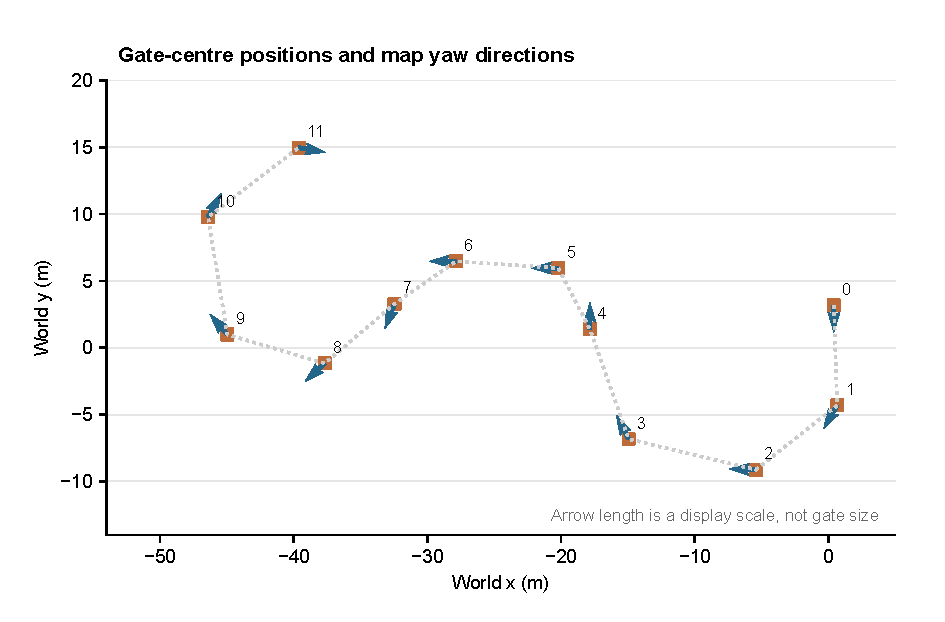
\includegraphics[width=\linewidth]{gate_headings.pdf}
\caption{Course waypoint geometry in the ROS world frame. Squares denote the
12 gate centres; arrows show the horizontal yaw directions extracted from the
converted quaternions. All arrows use the same display length. They do not encode
gate dimensions, and the dotted line is a waypoint-order guide.}
\label{fig:headings}
\end{figure}

\subsubsection{Part 0: first-gate reference}
The simple planner takes the first gate pose, normalises its quaternion and
publishes a desired state with zero linear and angular velocity and acceleration.
A 0.01\,s timer keeps the command active and broadcasts the desired pose in the
world frame. Empty lists and invalid first poses are rejected. The saved hover
record contains the position $(0.423,3.165,2.374)$\,m; this individual sample is
not used to estimate a settling time or a steady-state error statistic.

\subsubsection{Part 1.1: initialise from the current state}
The follower obtains position and yaw from \texttt{/current\_state} and waits
for a valid state before planning. Waypoints received first are retained until
that state arrives. The initial vertex is the measured position, which joins
the current vehicle location to the first gate. Once a trajectory exists, repeated
waypoint messages do not restart it.

\subsubsection{Part 1.2: optimise position and yaw}
The generator builds a three-dimensional position trajectory and a scalar yaw
trajectory using identical segment durations. Interior vertices constrain the
gate position and yaw. Successive yaw angles are unwrapped using
\begin{equation}
\psi_i=\psi_{i-1}+\operatorname{atan2}
\bigl(\sin(\bar\psi_i-\psi_{i-1}),\cos(\bar\psi_i-\psi_{i-1})\bigr),
\end{equation}
where $\bar\psi_i$ is the yaw extracted from the gate quaternion. This selects the
short angular increment across the $\pm\pi$ boundary.

Both optimisers minimise snap using ten coefficients per segment, so their
polynomials have degree at most nine. The library shares endpoint derivatives
through order four at interior vertices. Calls to
\texttt{makeStartOrEnd(..., SNAP)} set derivatives one through four to zero at
the overall endpoints. This implementation therefore includes endpoint snap
constraints and uses a different polynomial space from the minimal degree-seven
derivation in Deliverable 2. The mathematical count there applies to the stated
endpoint-through-jerk problem.

The segment-time estimator uses gate spacing with parameters $v_{\max}=2$\,m\,s$^{-1}$
and $a_{\max}=1$\,m\,s$^{-2}$. A time scale of 1 is applied and every segment is
at least 0.5\,s long. These parameters choose durations; the linear QP does not
impose them as hard velocity or acceleration bounds.

\subsubsection{Part 1.3: publish the desired state}
The generator evaluates position, velocity, acceleration, yaw, yaw rate and yaw
acceleration at the elapsed ROS time. The sample time is clipped to $[0,T]$, where
$T$ is the trajectory duration. The final rest reference therefore continues
after $T$. The desired-state timer is configured at 100\,Hz; the controller timer
is configured at 200\,Hz. These settings describe requested timer rates, not measured
throughput of the simulator.

\subsection{Experimental configuration and measurement}
The recorded experiment used the official Lab 4 Unity 2019.3.9f1 simulator with
Box64 0.3.6 on ARM64 and ROS Noetic. The selected controller gains were
$k_x=1.2$, $k_v=2.0$, $k_R=1.2$ and $k_\omega=0.7$, with drag compensation
disabled. State and desired-state timeout settings were both 1\,s. The saved
build log reports seven successfully built packages, and the saved integration
checks cover input validation, initial-state waiting, repeated waypoint messages,
yaw wrapping, derivative consistency and endpoint holding.

Results below use one recorded Unity run. The telemetry contains 6,064 rows;
each row pairs a current-state position with the latest received desired-state
position. This is the recorded online pairing, without subsequent temporal
interpolation. For sample $j$, the Euclidean tracking error is
\begin{equation}
e_j=\lVert\boldsymbol x_j-\boldsymbol x_{d,j}\rVert_2,\qquad
e_{\mathrm{RMS}}=\sqrt{\frac{1}{n}\sum_{j\in\mathcal A}e_j^2},
\end{equation}
where $\mathcal A$ contains the 4,556 samples whose reference time is below
$T-0.01$\,s and $n=|\mathcal A|$. The remaining 1,508 samples cover the terminal
reference hold. This distinction keeps the active-flight metric separate from
the terminal behaviour. All samples are retained in the time-series figures.

For gate $i$, the closest recorded centre distance and its time are
\begin{equation}
d_i=\min_j\lVert\boldsymbol x_j-\boldsymbol g_i\rVert_2,\qquad
t_i^{\mathrm{near}}=t_{\arg\min_j\lVert\boldsymbol x_j-\boldsymbol g_i\rVert_2}.
\end{equation}
Here $\boldsymbol g_i$ is the gate centre in ROS world coordinates. These are closest-approach times in the complete recording, including the final hold. The statistics describe 6,064 time samples within one run.

\subsection{Recorded flight through the course}
The trajectory and measured flight follow the sequence of all 12 gate centres
(Figure~\ref{fig:trajectory}). The reference lasts 91.0797\,s, while the full telemetry
record spans 121.30\,s. The terminal reference is first recorded at 91.16\,s on
the telemetry clock and remains active for the remaining 30.14\,s.

\begin{figure}[!htbp]
\centering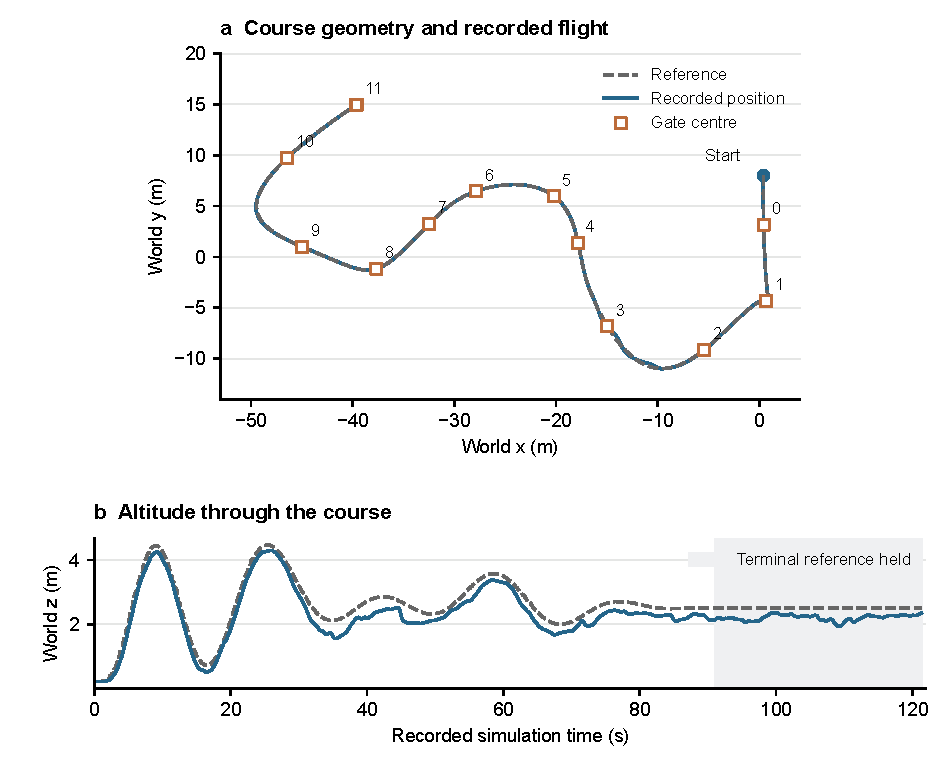
\includegraphics[width=\linewidth]{unity_trajectory.pdf}
\caption{Official Unity flight from the recorded telemetry. (a) Horizontal
projection of the reference and measured trajectory, with gate indices 0--11.
(b) Reference and measured altitude over the full recording. The shaded region
marks the terminal reference hold. All 6,064 samples are plotted; equal scaling
of the horizontal axes preserves course geometry.}
\label{fig:trajectory}
\end{figure}

The spatial view in Figure~\ref{fig:spatial} makes the vertical excursions visible
along the course. Figure~\ref{fig:axes} then separates the recorded and desired
coordinates so that changes in altitude can be compared with the horizontal motion.
\begin{figure}[!htbp]
\centering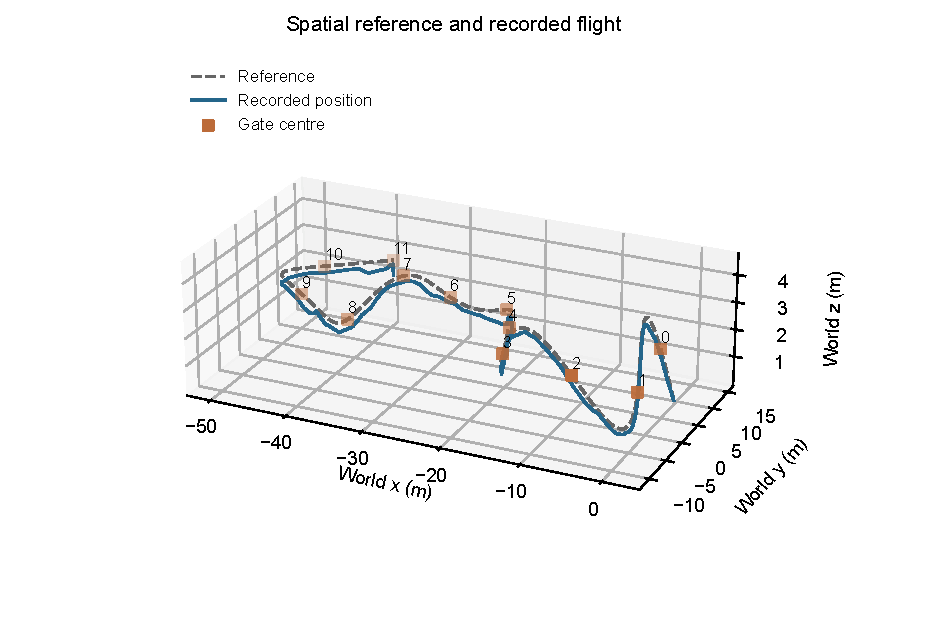
\includegraphics[width=\linewidth]{unity_3d.pdf}
\caption{Three-dimensional view of the recorded and reference trajectories,
with gate centres labelled 0--11. All telemetry samples are included. The vertical
display scale is enlarged relative to the horizontal axes to reveal changes in
altitude; tick labels retain physical distances in metres.}
\label{fig:spatial}
\end{figure}
\begin{figure}[!htbp]
\centering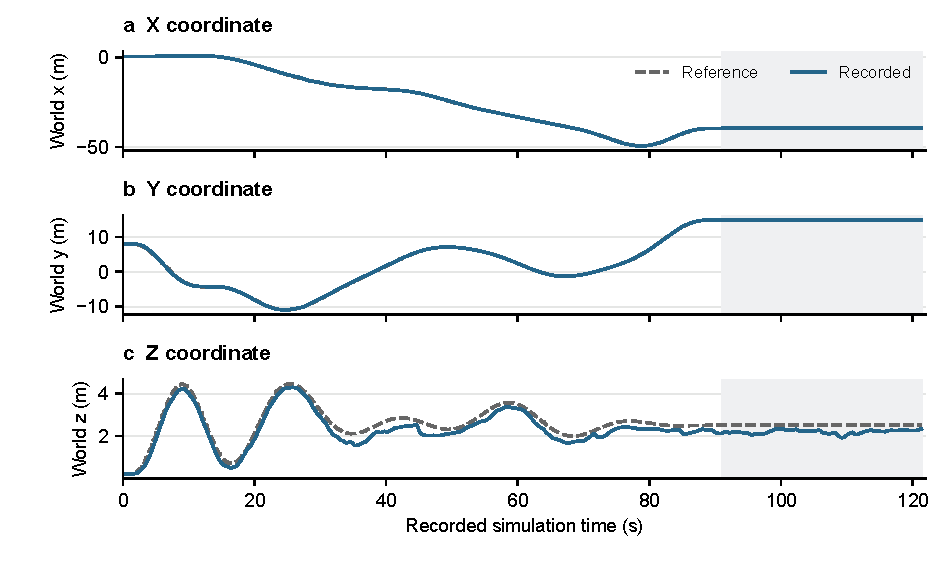
\includegraphics[width=\linewidth]{axis_tracking.pdf}
\caption{Coordinate-wise reference tracking through the complete recording.
The panels show world X, Y and Z positions, respectively. Dashed lines are references,
solid lines are recorded positions, and shading marks the terminal hold.
The panels use different position ranges, as labelled on their axes.}
\label{fig:axes}
\end{figure}

\begin{table}[htbp]
\centering\small
\caption{Measurements from the single recorded Unity run. Tracking statistics
use active-flight samples; final position error uses the last sample.}
\label{tab:metrics}
\begin{tabular}{@{}lr@{}}
\toprule
Quantity & Value\\\midrule
Reference trajectory duration & 91.0797\,s\\
Total telemetry duration & 121.30\,s\\
Active-flight RMS position error & 0.319\,m\\
Active-flight maximum position error & 0.578\,m\\
Largest closest-approach distance among the gates & 0.448\,m\\
Final position error relative to the last gate centre & 0.169\,m\\
Terminal-hold minimum / maximum position error & 0.151 / 0.585\,m\\
\bottomrule
\end{tabular}
\end{table}

\subsection{Tracking error and gate-centre visits}
The active-flight RMS error was 0.319\,m, with a maximum of 0.578\,m.
Figure~\ref{fig:errors} shows the complete error trace and the closest distance to every
gate. The closest-approach times increase strictly with gate index
(Table~\ref{tab:gates}), and each closest distance is below 0.45\,m. This 0.45\,m
value describes the observed distances; it is not a course-defined acceptance
threshold. Gates 4 and 5 have the largest closest distances, 0.445 and 0.448\,m.

The signed residuals in Figure~\ref{fig:signed} isolate the direction of the tracking
error. Their active-flight RMS values are 0.077\,m in X, 0.065\,m in Y and
0.303\,m in Z. The vertical component therefore makes the largest contribution
to the position error in this run. Figure~\ref{fig:distribution} summarises the
sample distribution: the active-flight median is 0.285\,m and the 95th percentile
is 0.507\,m. These are descriptive statistics of the recorded time samples.

\begin{figure}[!htbp]
\centering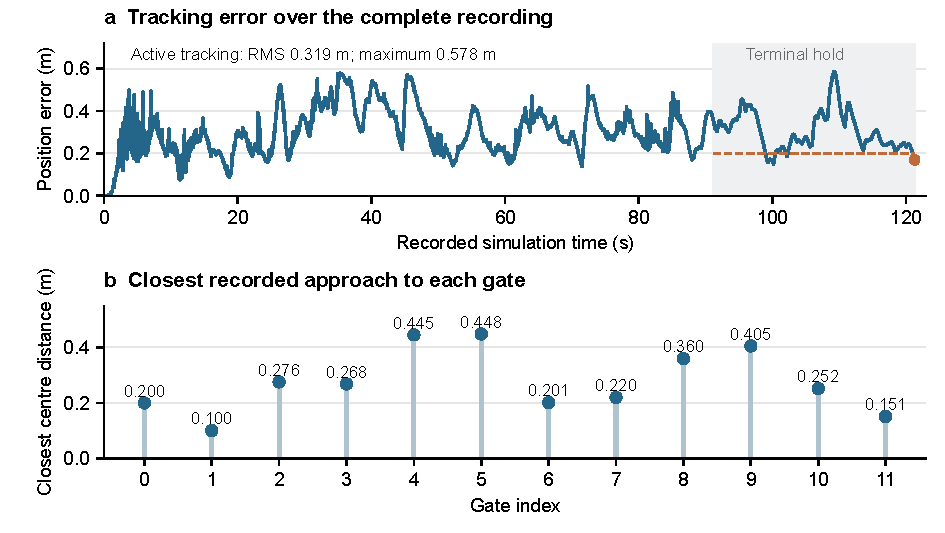
\includegraphics[width=\linewidth]{unity_errors.pdf}
\caption{Tracking accuracy and gate-centre proximity. (a) Euclidean error for
all recorded samples. The shaded interval is the terminal hold; the dashed
0.20\,m line is the local offline terminal tolerance, and the orange point is
the last sample. (b) Minimum Euclidean distance to each gate centre over the
complete recording. All measurements are from one Unity flight.}
\label{fig:errors}
\end{figure}

\begin{figure}[!htbp]
\centering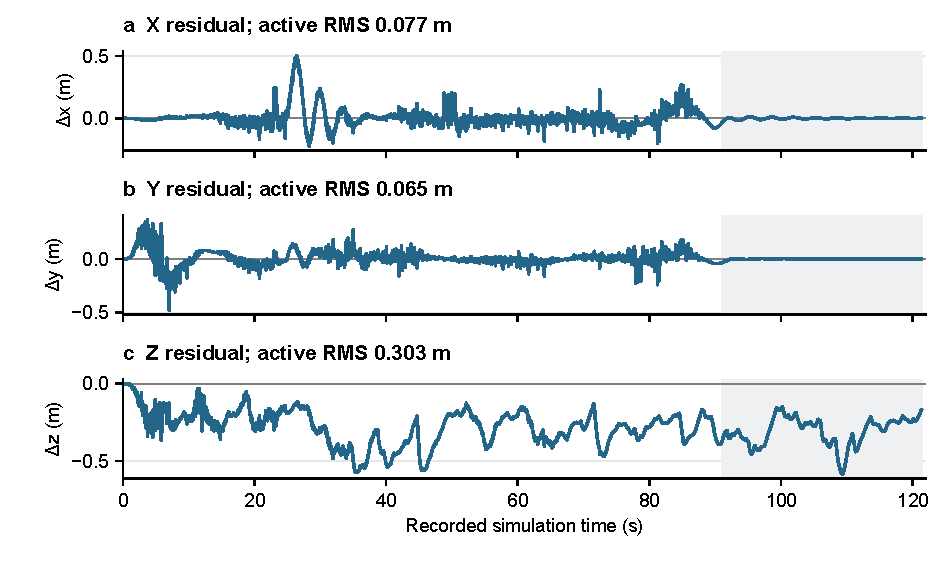
\includegraphics[width=\linewidth]{signed_errors.pdf}
\caption{Signed coordinate residuals, defined as recorded minus reference position.
Panel titles give the RMS over the 4,556 active-flight samples. All 6,064 samples
appear in the traces; shaded intervals mark the terminal hold. Individual axes
use separate vertical ranges to expose each component.}
\label{fig:signed}
\end{figure}
\begin{figure}[!htbp]
\centering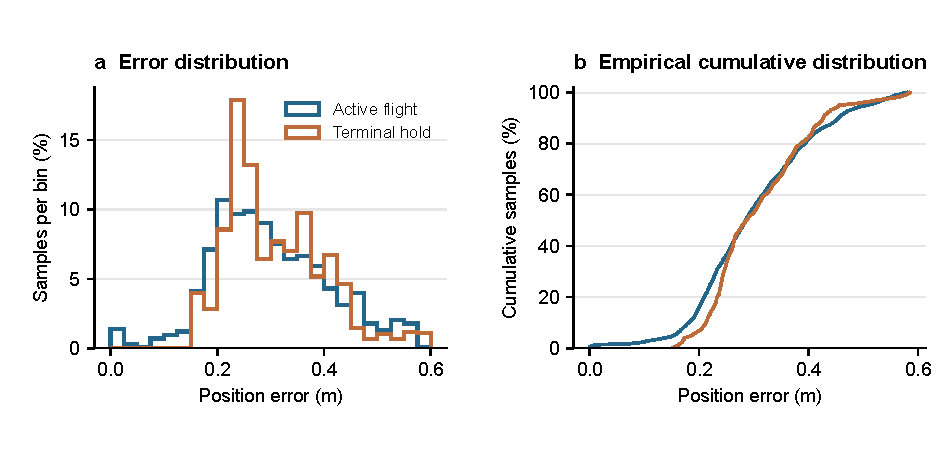
\includegraphics[width=\linewidth]{error_distribution.pdf}
\caption{Distribution of Euclidean tracking error. (a) Histograms with
0.025\,m bins, each normalised by the number of samples in its own phase.
(b) Empirical cumulative distributions using every sample in each phase.
The active and terminal phases contain 4,556 and 1,508 observations, respectively,
from the same flight.}
\label{fig:distribution}
\end{figure}

\begin{table}[htbp]
\centering\small
\caption{Closest-approach times and distances. Gate numbering follows the course
map. The final gate's closest approach occurs during the terminal hold.}
\label{tab:gates}
\begin{tabular}{@{}rrr@{\hspace{10mm}}rrr@{}}
\toprule
Gate & Time (s) & Distance (m) & Gate & Time (s) & Distance (m)\\\midrule
0 & 5.72 & 0.200 & 6 & 52.94 & 0.201\\
1 & 13.02 & 0.100 & 7 & 58.82 & 0.220\\
2 & 21.18 & 0.276 & 8 & 65.86 & 0.360\\
3 & 30.82 & 0.268 & 9 & 73.64 & 0.405\\
4 & 39.66 & 0.445 & 10 & 82.46 & 0.252\\
5 & 44.88 & 0.448 & 11 & 100.18 & 0.151\\\bottomrule
\end{tabular}
\end{table}

\subsection{Recorded attitude and terminal response}
Figure~\ref{fig:attitude} adds the attitude history from the recorded quaternions.
After normalisation, each quaternion is converted to roll, pitch and yaw using
the ZYX Euler-angle convention. Yaw is unwrapped in time to keep the displayed
heading continuous across the angular representation boundary. The plot reports
the measured attitude; the CSV does not contain a desired-attitude series for
an attitude-error comparison.
\begin{figure}[!htbp]
\centering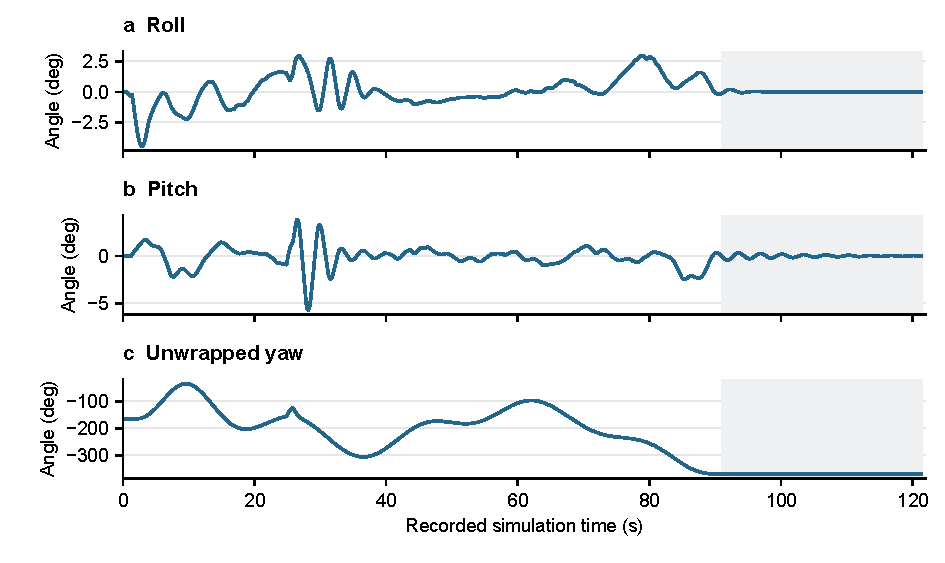
\includegraphics[width=\linewidth]{recorded_attitude.pdf}
\caption{Recorded roll, pitch and unwrapped yaw in degrees. Angles are derived
from all 6,064 recorded quaternions, using the normalised $(x,y,z,w)$ components
and a ZYX convention. Yaw can extend outside $[-180,180]$ degrees after unwrapping.
The shaded interval marks the terminal reference hold.}
\label{fig:attitude}
\end{figure}

Figure~\ref{fig:terminal} enlarges the terminal interval. Time is reset to zero
at the first telemetry row classified as terminal hold. The altitude trace
shows the vertical response against the fixed final reference while the upper
panel retains the full Euclidean position error.
\begin{figure}[!htbp]
\centering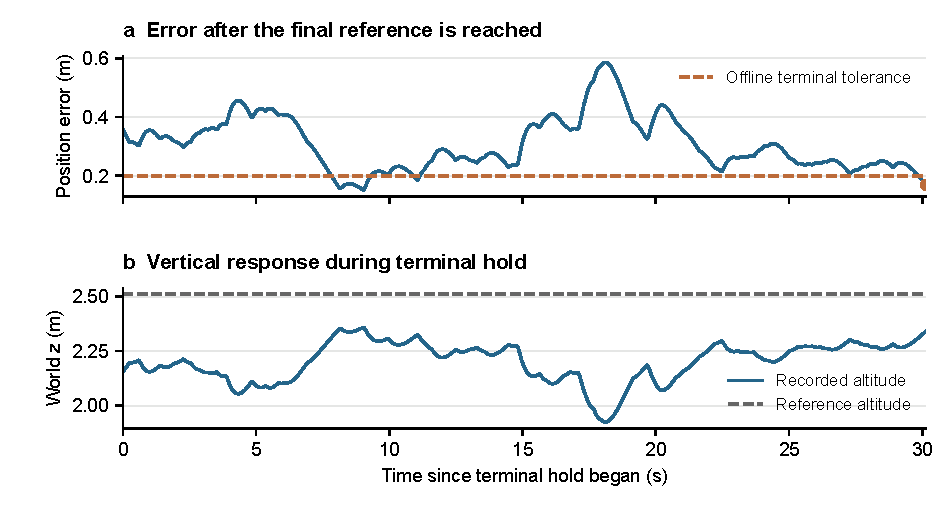
\includegraphics[width=\linewidth]{terminal_detail.pdf}
\caption{Detailed terminal response over all 1,508 hold samples. (a) Position
error relative to the held reference; the dashed line is the offline 0.20\,m
terminal tolerance and the point marks the final sample. (b) Actual and reference
altitude. The time axis begins at recorded simulation time 91.16\,s.}
\label{fig:terminal}
\end{figure}

\noindent\begin{minipage}{\linewidth}
The last position was 0.169\,m from the final gate centre. Over the terminal
hold, the error ranged from 0.151 to 0.585\,m, so the final sample satisfies
the offline 0.20\,m tolerance without establishing that the entire hold stayed
inside it. The original live-monitor log ended with a failed completion check;
the accompanying run notes identify its threshold as 0.08\,m. The later offline
check uses 0.20\,m. Reporting the trace and final distance preserves the measured
outcome independently of either threshold.
\end{minipage}



\subsection{Simulator view and terminal behaviour}
The retained simulator screenshot in Figure~\ref{fig:unity} places the telemetry in its
visual context. It shows the quadrotor near a green gate with additional gates
visible along the course. The saved screen recording and rosbag accompany this
report locally. The bag metadata records 6,284 current-state messages and 3,125
desired-state messages over approximately 125\,s; its recording starts before the
paired telemetry series, so the durations and sample counts differ.

\begin{figure}[!htbp]
\centering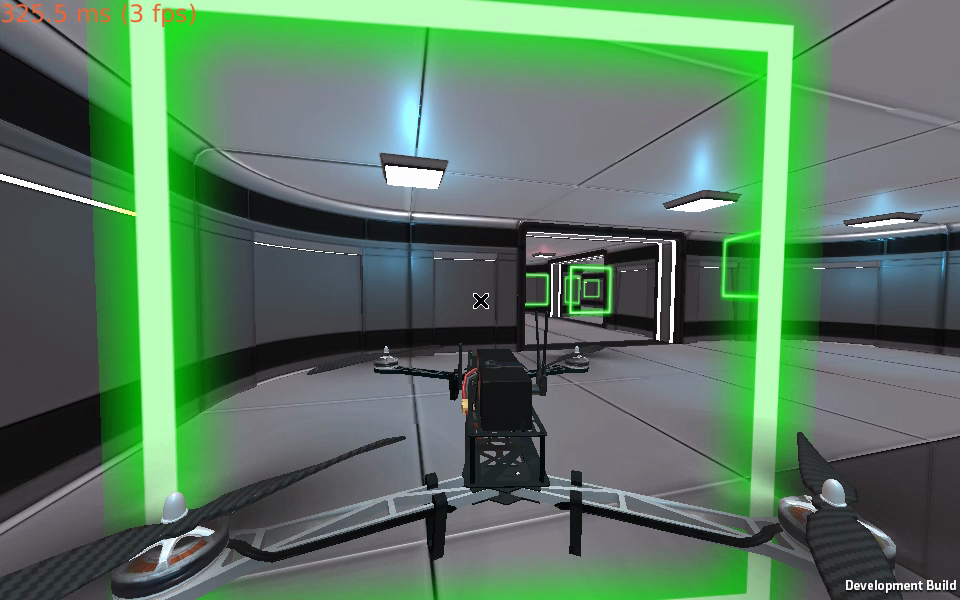
\includegraphics[width=.78\linewidth]{unity_final_gate.png}
\caption{Retained view from the official Unity experiment. The screenshot is
reproduced in full, with its original colours and aspect ratio. It supplies scene
context for the trajectory plots; the gate-centre distances come from telemetry.}
\label{fig:unity}
\end{figure}

Figures~\ref{fig:videoearly} and~\ref{fig:videolate} sample the saved video at
10\,s playback intervals, starting at 5\,s. They show the progression of the
rendered course and the later views near the terminal gate. Their labels refer
to video playback time, which has not been synchronised with the telemetry clock.
Frames retain their full area in chronological order.
\begin{figure}[!htbp]
\centering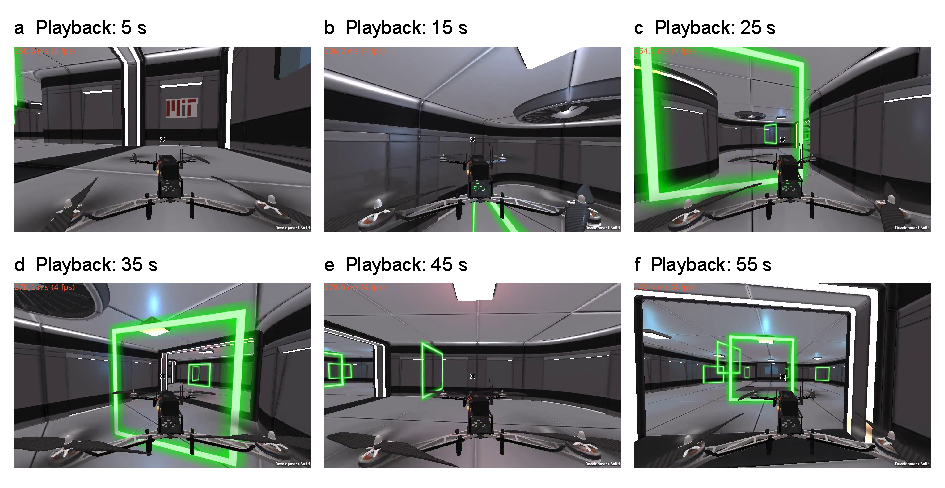
\includegraphics[width=\linewidth]{video_sequence_1.pdf}
\caption{First six sampled views from the official Unity screen recording,
at requested playback times 5, 15, 25, 35, 45 and 55\,s. Each panel is a decoded
960$\times$600 frame, scaled without cropping or colour adjustment. These
playback times are distinct from the simulation timestamps on the data plots.}
\label{fig:videoearly}
\end{figure}
\begin{figure}[!htbp]
\centering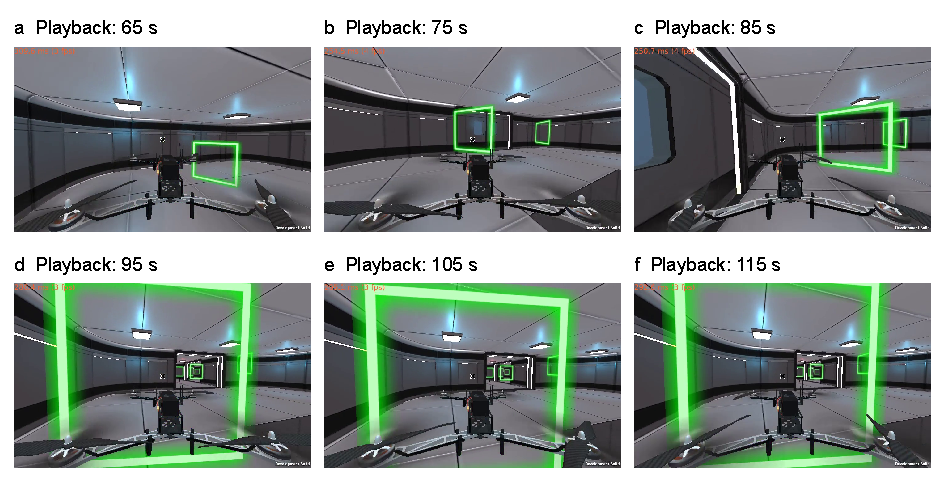
\includegraphics[width=\linewidth]{video_sequence_2.pdf}
\caption{Later sampled views from the same recording, at requested playback
times 65, 75, 85, 95, 105 and 115\,s. Panels retain their original framing and
colours. The final views document the scene near the terminal gate; no gate-event
timestamps are inferred from this evenly spaced video sample.}
\label{fig:videolate}
\end{figure}





Appendix~\ref{sec:gateatlas} provides a visual record for every gate, with
complete centre-distance histories and local trajectory projections around the
closest recorded approach.

\section{Discussion}
\subsection{Polynomial freedom and boundary conditions}
The single-segment solutions show when a higher polynomial degree is useful.
With position constraints alone, constant velocity already reaches the global
lower bound. The terminal-velocity condition changes the feasible set: a cubic
can redistribute velocity over the interval and reduce the cost from 4 to $17/8$.
The overshoot in Figure~\ref{fig:single} follows from arriving at the final point with
negative velocity. Boundary conditions therefore determine the value of extra
coefficients more directly than polynomial degree alone.

For multiple segments, the distinction between explicit constraints and natural
conditions explains how the optimiser chooses free waypoint derivatives. In the
flight implementation, shared position and yaw segment times keep the reference
components synchronised, while angle unwrapping avoids a full-turn interpolation
at a representation discontinuity. Endpoint sampling then gives the controller
a persistent rest reference after the planned motion ends.

\subsection{What the flight measurements establish}
The recorded run supports ordered gate-centre visits and quantifies tracking over
the course. Centre proximity is a spatial diagnostic: a collision-free crossing
of every gate would require crossing geometry or simulator event records in
addition to these distances. Likewise, 91.08\,s is the reference duration, not an
independently measured official race time. The optional speed challenge is outside
the demonstrated result.

The terminal trace shows continued position variation after the reference stops.
A time-window settling criterion would be needed to quantify sustained hover
accuracy. No controller comparison is available to attribute that variation to
a particular gain, bridge timing effect or simulator model. The present results
therefore describe the selected configuration and recorded run. They provide
a concrete starting point for any subsequent time-allocation or gain study.

\section{Conclusions}
The analytical exercises connect polynomial coefficients to boundary conditions
and identify the continuity and stationarity conditions for multi-segment planning.
The implemented ROS follower extends that formulation to spatial waypoints and
unwrapped yaw, then supplies the derivatives needed by the Lab 3 controller.
In the official Unity recording, the vehicle approached all 12 gate centres in
order with an active-flight RMS position error of 0.319\,m. Together, the
derivations and recorded flight demonstrate the complete chain from waypoint
constraints to a tracked reference trajectory.

\begingroup\small\setlength{\bibsep}{2pt}\begin{thebibliography}{9}
\bibitem{lab4} MIT Visual Navigation for Autonomous Vehicles.
\emph{Lab 4: Exercises}, 2023 course materials.
\url{https://vnav.mit.edu/labs_2023/lab4/exercises.html}.
Accessed 10 October 2026.
\bibitem{mavlib} ETH Zurich Autonomous Systems Lab.
\emph{mav\_trajectory\_generation: Polynomial trajectory generation and optimisation}.
\url{https://github.com/ethz-asl/mav_trajectory_generation}.
Library documentation and the implementation distributed with the laboratory.
Accessed 10 October 2026.
\end{thebibliography}\endgroup

\appendix
\section{Per-gate trajectory views}
\label{sec:gateatlas}
Figures~\ref{fig:gdistfirst} and~\ref{fig:gdistlast} retain the complete time
history of distance to each of the 12 centres. The minima progress in gate order.
Figures~\ref{fig:glocalfirst} and~\ref{fig:glocallast} show the local geometry
within two seconds before and after each minimum, giving 201 samples per gate.
Every gate is included with the same time-window rule and plotting scale.



\begin{figure}[!htbp]
\centering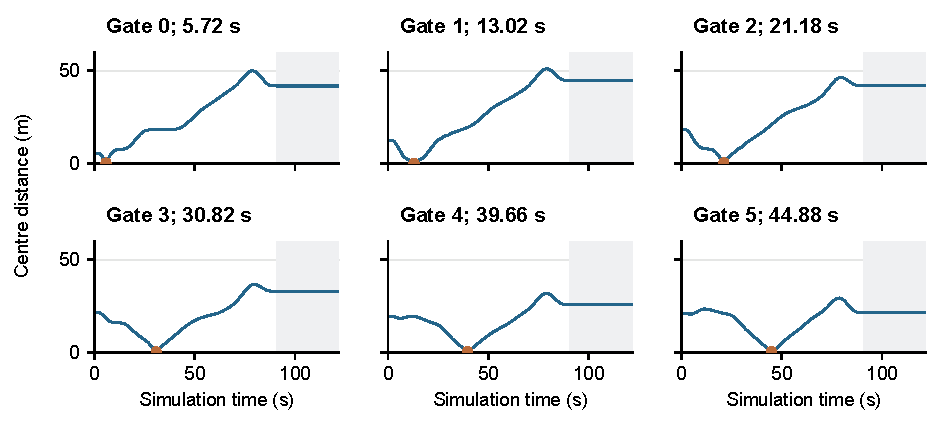
\includegraphics[width=\linewidth]{gate_distances_00_05.pdf}
\caption{Complete centre-distance histories for gates 0--5. Each panel includes
all 6,064 telemetry samples and uses the same axes. Orange points mark the global
minimum for each gate; shading marks the terminal reference hold.}
\label{fig:gdistfirst}
\end{figure}
\begin{figure}[!htbp]
\centering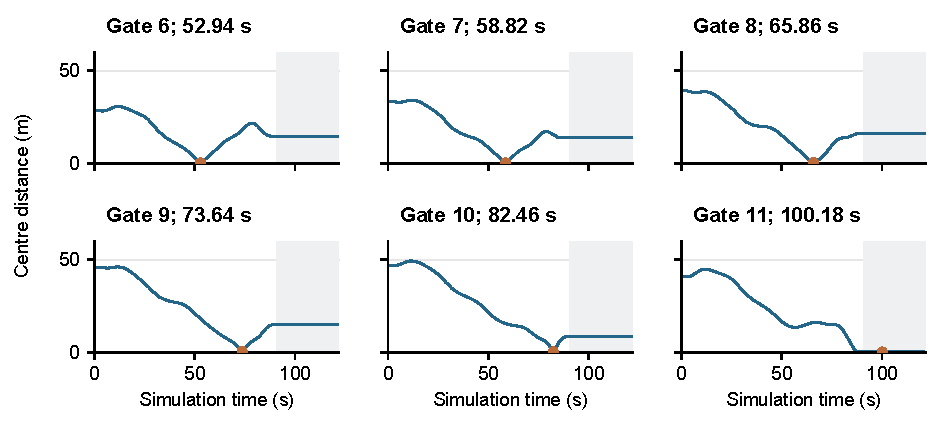
\includegraphics[width=\linewidth]{gate_distances_06_11.pdf}
\caption{Complete centre-distance histories for gates 6--11, using the same
sample set and scales as Figure~\ref{fig:gdistfirst}. The last gate's global
minimum occurs during the terminal hold.}
\label{fig:gdistlast}
\end{figure}
\subsection{Local trajectory projections}
For the local views, $s=\cos\psi_i(x-x_i)+\sin\psi_i(y-y_i)$ is the horizontal
offset projected along the map yaw of gate $i$, and the vertical coordinate is
$z-z_i$. The square is the gate centre. The perpendicular horizontal coordinate
is omitted from this two-dimensional projection, so the minimum distance in each
title is still computed from the full three-dimensional position. These plots
show local tracking geometry without assuming an unrecorded gate-opening size.

\begin{figure}[!htbp]
\centering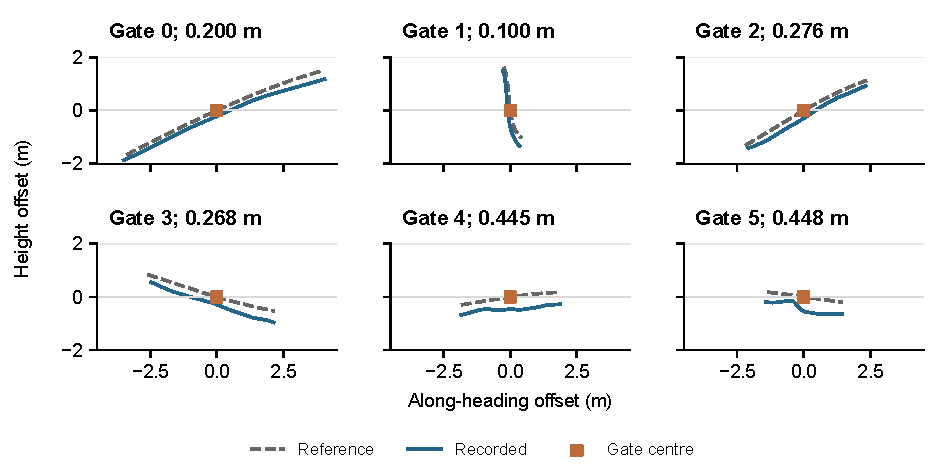
\includegraphics[width=\linewidth]{gate_local_00_05.pdf}
\caption{Local views around the closest approaches to gates 0--5. Each panel
contains the 201 samples within $\pm2$\,s of that gate's minimum-distance time.
Both axes show offsets in metres with equal scale; reference and recorded
positions are projected onto along-heading offset and height. The square denotes
the centre, and the title reports the minimum full 3D distance.}
\label{fig:glocalfirst}
\end{figure}
\begin{figure}[!htbp]
\centering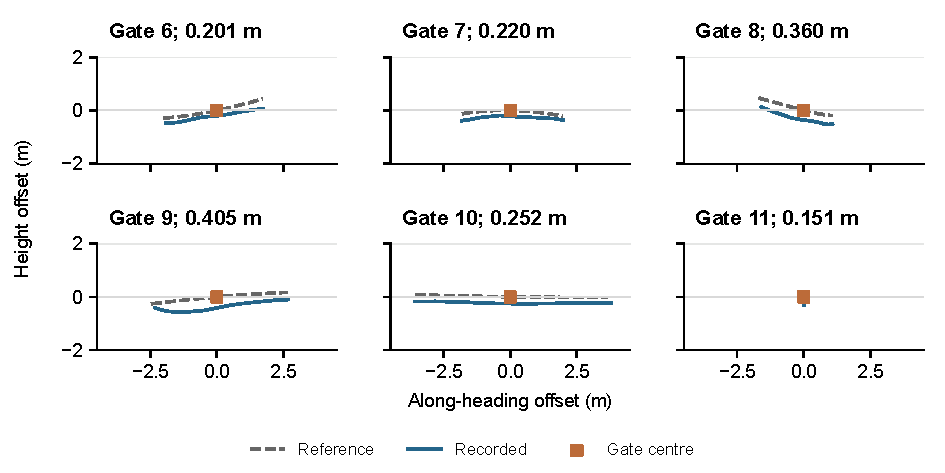
\includegraphics[width=\linewidth]{gate_local_06_11.pdf}
\caption{Local views for gates 6--11 using the same window and coordinate
definitions as Figure~\ref{fig:glocalfirst}. Gate 11's window lies in the terminal
hold, where horizontal motion is small and the remaining variation is mostly vertical.}
\label{fig:glocallast}
\end{figure}
\end{document}
